\title{LEZIONE 8 21/04/2020}\newline
\textbf{link} \href{https://web.microsoftstream.com/video/daf8e418-03bf-40c5-8093-3391c41375be}{clicca qui}
\section{Dinamica dei corpi rigidi}
\subsection{Baricentro}
\subsubsection{Masse puntiformi}
Introduciamo per prima cosa il concetto di baricentro per \textbf{masse puntiformi}, in seguito estenderemo il concetto per le masse di corpi rigidi
[immagine dagli appunti del prof]
\begin{center}
    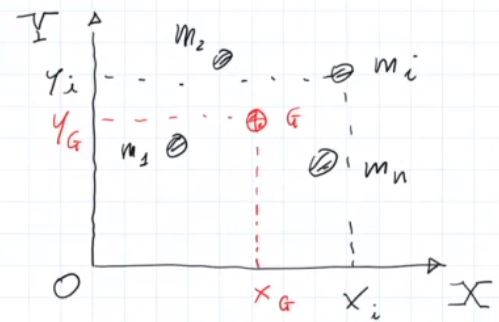
\includegraphics[height=3cm]{../lezione8/img1.JPG}
\end{center}
Detto $G$ il \textbf{baricentro}, esso ha due coordinate $x_G$ e $y_G$, definite come media pesata delle coordinate di tutte le masse puntiformi in gioco, dove il peso è dato dalla massa del singolo punto:
\[
    \begin{cases}
        x_G = \frac{\sum_{i=1}^{n} x_i m_i}{m}\\
        y_G = \frac{\sum_{i=1}^{n} y_i m_i}{m}
    \end{cases}
\]
dove $m = \sum_{i=1}^{n} m_i$.\newline
\newline
Le coordinate del baricentro possono anche essere definite come
\[
    \begin{cases}
        x_G = \frac{S_y}{m}\\
        y_G = \frac{S_x}{m}
    \end{cases}
\]
dove $S_y = \sum_{i=1}^{n} x_i m_i$ e $S_x = \sum_{i=1}^{n} y_i m_i$ sono i \textbf{momenti statici del prim'ordine} attorno, rispettivamente, all'asse $Y$ e all'asse $X$.\newline
\newline
Possiamo dire che  il baricentro $G$ è il \textbf{centro delle forze peso}, questo significa che il momento del baricentro delle forze peso rispetto al polo $G$ è nullo.\subsubsection{Copri rigidi}
Per estendere il concetto ddi baricentro ai \textbf{corpi rigidi} ci basta considerare il corpo rigido come un insieme infinito e continuo di infiniti punti.\newline
\newline
[immagine dagli appunti del prof]
\begin{center}
    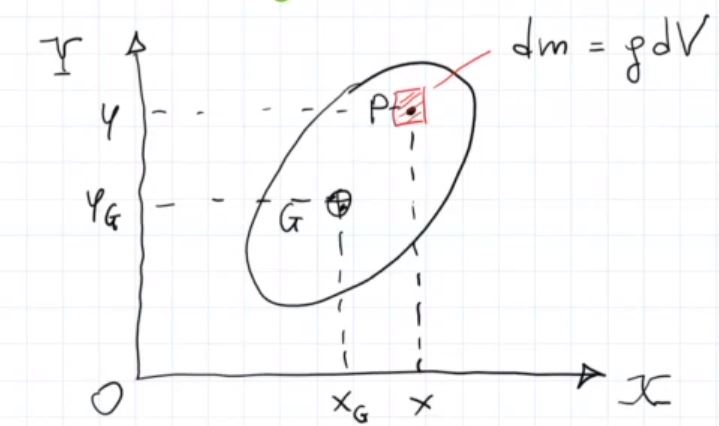
\includegraphics[height=3cm]{../lezione8/img2.JPG}
\end{center}
Definito un corpo rigido e una piccola sezione infinitesima di massa $dm = \rho dV $, con $\rho$ densità. Considerando che l'intero corpo è costituito da infiniti punti, per calcolare le coordinate del baricentro è sufficiente sostituire la sommatoria con un integrale:
\[
    \begin{cases}
        x_G = \frac{1}{m} \int_V \rho (x,y,z) x dV\\
        y_G = \frac{1}{m} \int_V \rho(x,y,z) y dV
    \end{cases}
\]
Notiamo che se si sceglie un \textbf{sistema di riferimento baricentrico} cioè con origine nel baricentro, allora i momenti statici del prim'ordine si annullano.\newline
\newline
Se, inoltre, definiamo dei corpi rigidi \textbf{omogenei}, cioè con densità costante $\rho(x,y,z) = \rho = costante$ e di \textbf{spessore costante} (spessore uscente dal foglio) $h = costante$, allora $dV = h dA$ e quindi il calcolo delle coordinate si semplifica molto:
\[
    x_G = \frac{\rho h}{m} \int_{A} x dA = \frac{1}{A} \int_{A} x dA\\
    y_G = \frac{\rho h}{m} \int_{A} y dA = \frac{1}{A} \int_{A} y dA
\]
Da qui notiamo che in caso di corpi rigidi omogenei e di spessore costante possiamo studiarne il baricentro analizzandone la geometria:
\begin{itemize}
    \item Se il corpo possiede un asse di simmetria, allora il baricentro dovrà appartenere a questo asse;
    \item Se un corpo ha più di un asse di simmetria, allora il baricentro si troverà sull'intersezione di questi;
    \item Se un corpo è facilmente suddivisibile in sottocorpi di cui è noto il baricentro, allora la posizione del baricentro del corpo intero sarà la media pesata dei baricentri dei sottocorpi.
\end{itemize}
\subsection{Momento di inerzia}
\subsubsection{Masse puntiformi}
Il \textbf{momento di inerzia} ci dice come la massa sia distribuita all'interno del corpo.\newline
\newline
[immagine dagli appunti del prof]
\begin{center}
    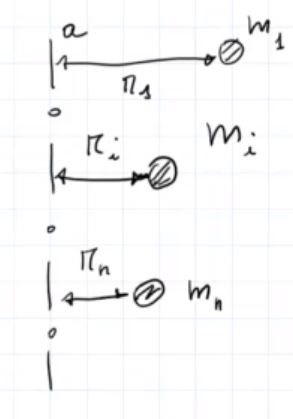
\includegraphics[height=4cm]{../lezione8/img3.JPG}
\end{center}
Dato un asse $a$ (tratteggio-puntini nell'immaigne), date delle masse $m_i$ puntiformi, allora il momento di inerzia $J_a$ è dato dal \textbf{momento statico del secondo ordine} ($= \sum m_i r_i^2$)  della massa rispetto all'asse $a$:
\[
    J_a = \sum_{i=1}^{n} m_i r_i^2
\]
Tanto più una massa è distante dall'asse tanto più sarà grande il suo momento di inerzia.\newline
\newline
Nel caso piano, l'unico asse di nostro interesse sarà un asse perpendicolare all'asse del foglio, come l'asse $z$.
\subsubsection{Corpo rigido}
Vediamo il caso di corpo rigido:\newline
[immagine dagli appunti del prof]
\begin{center}
    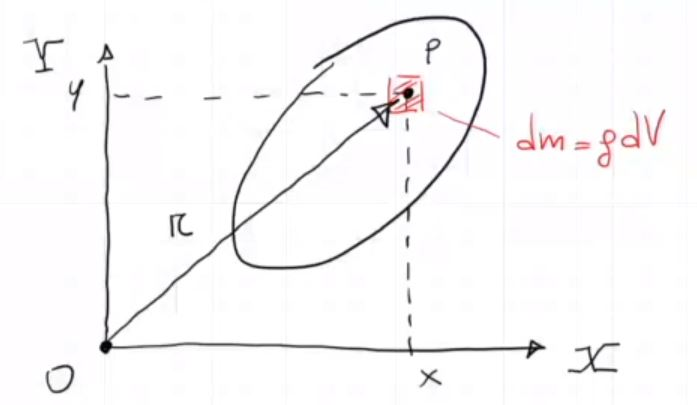
\includegraphics[height=3cm]{../lezione8/img4.JPG}
\end{center}
Dato un punto $P$ appartente al copro rigido e che ha una massa infinitesima $dm = g dV$, per estendere il concetto da massa puntiforme a corpo rigido, tutto quello che dobbiamo fare è sostituire il simbolo di sommatoria con quello di integrale.\newline
\newline
In questo corso studieremo sempre il momento di inerzia in riferimento all'asse $z$, e quindi per indicare il momento di inerzia $J_{OZ}$, cioè per l'asse $Z$ e il polo $O$ (origine), per comodità scriveremo solo $J_O$:
\[
    J_{O} = \int_V \rho(x,y,z) r^2 dV = \int_V \rho(x,y,z) (x^2+y^2) dV
\]
\ \newline
Vediamo ora il caso di un corpo \textbf{omogeneo} e a \textbf{spessore costante}:
\[
    J_O = \int_V \rho(x^2+y^2) dV = \int_A \rho h(x^2 + y^2) dA = \rho h \int_A r^2 dA
\]
\ \newline
Il momento di inerzia di un corpo diventa una \textbf{caratteristica del corpo} quando lo si considera per il polo $G$, cioè per il baricentro. In questo caso più la massa è lontana dal baricentro più il momento di inerzia è maggiore.\newline
Se si sceglie un qualsiasi altro polo, il momento di inerzia non è più una proprietà del corpo, perchè dipende dal polo scelto.\newline
\newline
Come possiamo legare il momento di inerzia di un generico polo $O$ rispetto al momento di inerzia del baricentro?\newline
\textbf{Teorema del trasporto o teroema di Huygens}:
\[
    J_O = J_G + m \bar{OG}^2 \;\;\;[Kg m^2]
\]
con $m$ massa del corpo e $\bar{OG}$ distanza del generico polo $O$ dal baricentro $G$.
\newline
\newline
Vediamo come dimostrarlo:\newline
[immagine dagli appunti del prof]
\begin{center}
    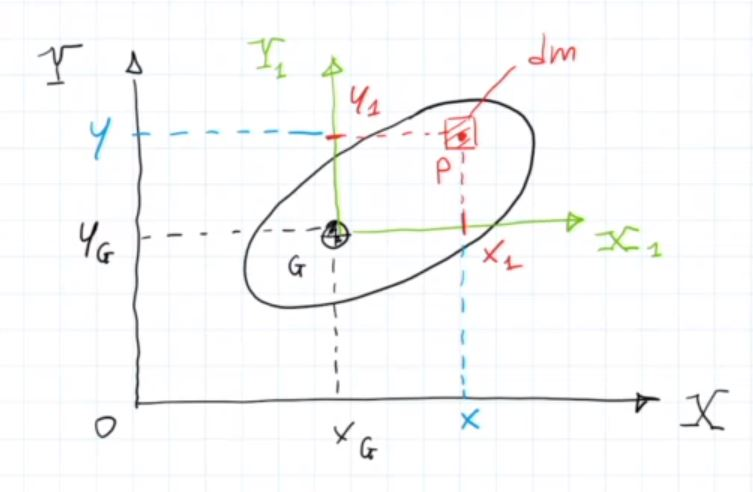
\includegraphics[height=3cm]{../lezione8/img5.JPG}
\end{center}
\[
    J_O = \int_V \rho(x^2 + y^2) dV = \int_V \rho [(x_G + x_1)^2 + (y_G + y_1)^2] dV = 
\]
\[
    = \int_V \rho(x_G^2 + y_G^2) dV + \int_V \rho(x_1^2 + y_1^2) dV + 2 \int_V \rho x_G x_1 dV + 2 \int_V \rho y_Gy_1 dV = 
\]
\[
    = (x_G^2 + y_G^2)\int_V \rho dV + \int_V \rho(x_1^2 + y_1^2) dV + 2 x_G  \int_V \rho  x_1 dV + 2 y_G \int_V \rho y_1 dV = J_G + m \bar{OG}^2
\]
\ \newline
\textbf{es.} Trave rettangolare omogenea a spessore costante. \newline
[immagine dagli appunti del prof]
\begin{center}
    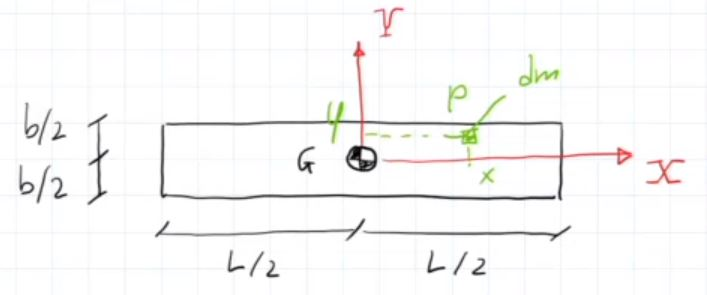
\includegraphics[height=3cm]{../lezione8/img6.JPG}
\end{center}
\[
    J_G = \rho h \int_A (x^2 + y^2) dA
\]
\[
    J_G = \rho h \int_{- \frac{b}{2}}^{\frac{b}{2}} \int_{- \frac{b}{2}}^{\frac{b}{2}} (x^2 + y^2) dy dx = \rho h \int_{- \frac{b}{2}}^{\frac{b}{2}} \int_{- \frac{b}{2}}^{\frac{b}{2}} x^2 dx dy + gh \int_{- \frac{b}{2}}^{\frac{b}{2}} \int_{- \frac{b}{2}}^{\frac{b}{2}} y^2 dx dy
\]
\[
    J_G = \rho h b \left[\frac{x^3}{3}\right]_{- \frac{b}{2}}^{\frac{b}{2}} + \rho h L \left[\frac{y^3}{3}\right]_{- \frac{b}{2}}^{\frac{b}{2}}
\]
\[
    J_G = \rho h b \left(\frac{L^3}{24} + \frac{L^3}{24}\right) + \rho h L \left( \frac{b^3}{24} + \frac{b^3}{24}\right)
\]
Se la trave fosse stata snella avremmo semplificato ulteriormente:
\[
    L >> b \Rightarrow J_G \tilde{=} \frac{m}{12} L^2
\]
\rule{\textwidth}{0,4pt}
\ \newline
Notiamo che possiamo sempre in generale scrivere il momento di inerzia di un corpo come il prodotto fra la massa $m$ e il \textbf{raggio giratorio di inerzia} $r_G$ al quadrato:
\[
    J_G = m r_G^2
\]
\ \newline
Nel caso della trave snella dell'esempio precedente notiamo che il raggio giratorio di inerzia è pari a $L$.\newline
\newline
Il raggio giratorio di inerzia ci dice quanto la massa è concentrata intorno al baricentro del corpo, quanto più è piccolo e quanto più la massa è concentrata vicino al baricentro.
\newline
\newline
\textbf{es.} Corona circolare omogenea a spessore costante.\newline
[immagine dagli appunti del prof]
\begin{center}
    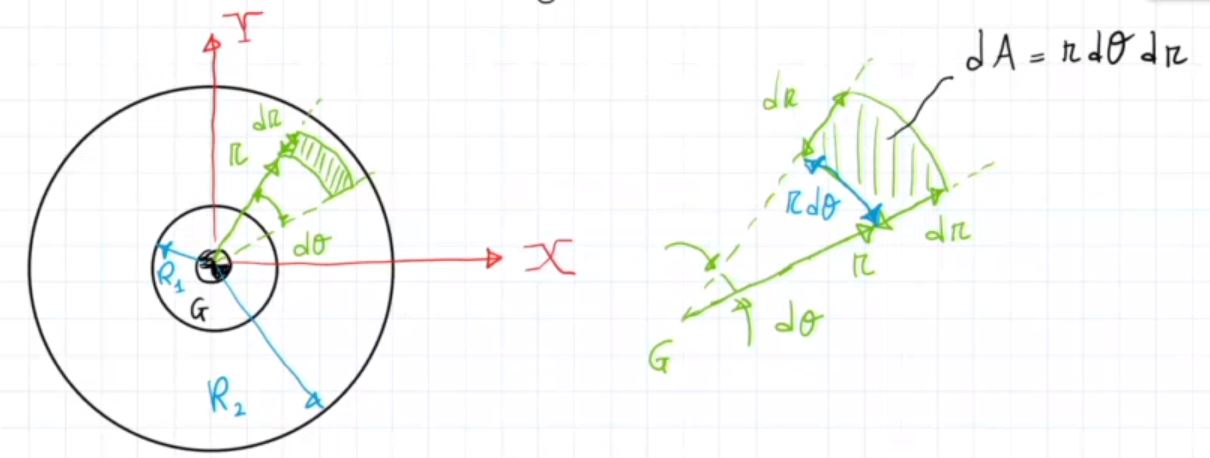
\includegraphics[height=3cm]{../lezione8/img7.JPG}
\end{center}
Consideriamo un settore circolare di apertura infinitesima $d \theta$ e di spessore infinitesimo $d r$ e che quindi avrà area approsismabile a un rettangolo $dA = r d \theta d r$ e la generica distanza dal punto $x^2 + y^2 = r^2$:
\[
    J_G = \rho h \int_A (x^2 + y^2) dA = \rho h \int_{0}^{2\pi} \int_{R_1}^{R_2} r^2 r d r d \theta = \rho h \int_{0}^{2\pi} \int_{R_1}^{R_2} r^3 d r d \theta
\]
\[
    J_G = 2 \pi \rho h \int_{R_1}^{R_2} r^3 dr = 2 \pi \rho h \left[\frac{r^4}{4}\right]_{R_1}^{R_2} = \pi \rho h \frac{R_2^4 - R_1^4}{2} = \rho \frac{\pi h }{2} (R_2^2 + R_1^2) (R_2^2 - R_1^2)
\]
notiamo che l'area della corona circolare è $A = \pi (R_2^2 -R_1^2)$ e che $V = A h$ e $m = \rho V$, per cui:
\[
    J_G = \frac{m}{2}(R_2^2 + R_1^2)
\]
Introduciamo ora il raggio giratorio di inerzia:
\[
    J_G = m r_G^2
\]
e mostriamo due casi separati:
\begin{itemize}
    \item Anello sottile, in cui tutta la massa è concetrata sull'anello esterno: $J_G = m R^2$, per cui $r_G = R$.
    \item Disco pieno, in cui l'intero disco possiede massa: in questo caso la massa va dal raggio $R_1= 0$ al raggio $R_2 = R$ e quindi $J_G = m \frac{R^2}{2}$ e $r_G = \frac{\sqrt{2}}{2}R$.
\end{itemize}
Da questo esempio notiamo che il raggio giratorio di inerzia ci mostra la distribuzione della massa rispetto al baricentro.\newline
\rule{\textwidth}{0,4pt}